\chapter{Background and State of the art}


\todo{Wasm and portable code}
    \todo{How => Why: Motivation, security, reliability}
\todo{Diversification, Superoptimization and Superdiversification.}
    \todo{Prexisting => Artificial}
    \todo{How => Why: Motivation, security, reliability}
    \todo{Fuzzing (CVE)}
\todo{Randomization (runtime).}
    \todo{N-version, Isomeron eg}
    \todo{How => Why: Motivation, security, reliability}
\todo{1 - page MEWE and << CROW (Our contributions)}
    \todo{n-variant}

\section{CROW}
\label{section:crow}

\begin{comment}
This section describes CROW, a tool tailored to create semantically equivalent variants out of a single program, either C/C++ code or LLVM bitcode. We assume that the \wasm programs are generated through the LLVM compilation pipeline to implement CROW. This assumption is supported by the work of Lehman et al. \cite{}; the fact that LLVM-based compilers are the most popular compilers to build \wasm programs \cite{usenixWASM2020} and the availability of source code (typically C/C++; and LLVM for \wasm) that provides a structure to perform code analysis and produce code replacements that is richer than the binary code. CROW is part of the contributions of this thesis.
In \autoref{diagrams:crow}, we describe the workflow of CROW to create program variants.

\begin{figure*}[h]
    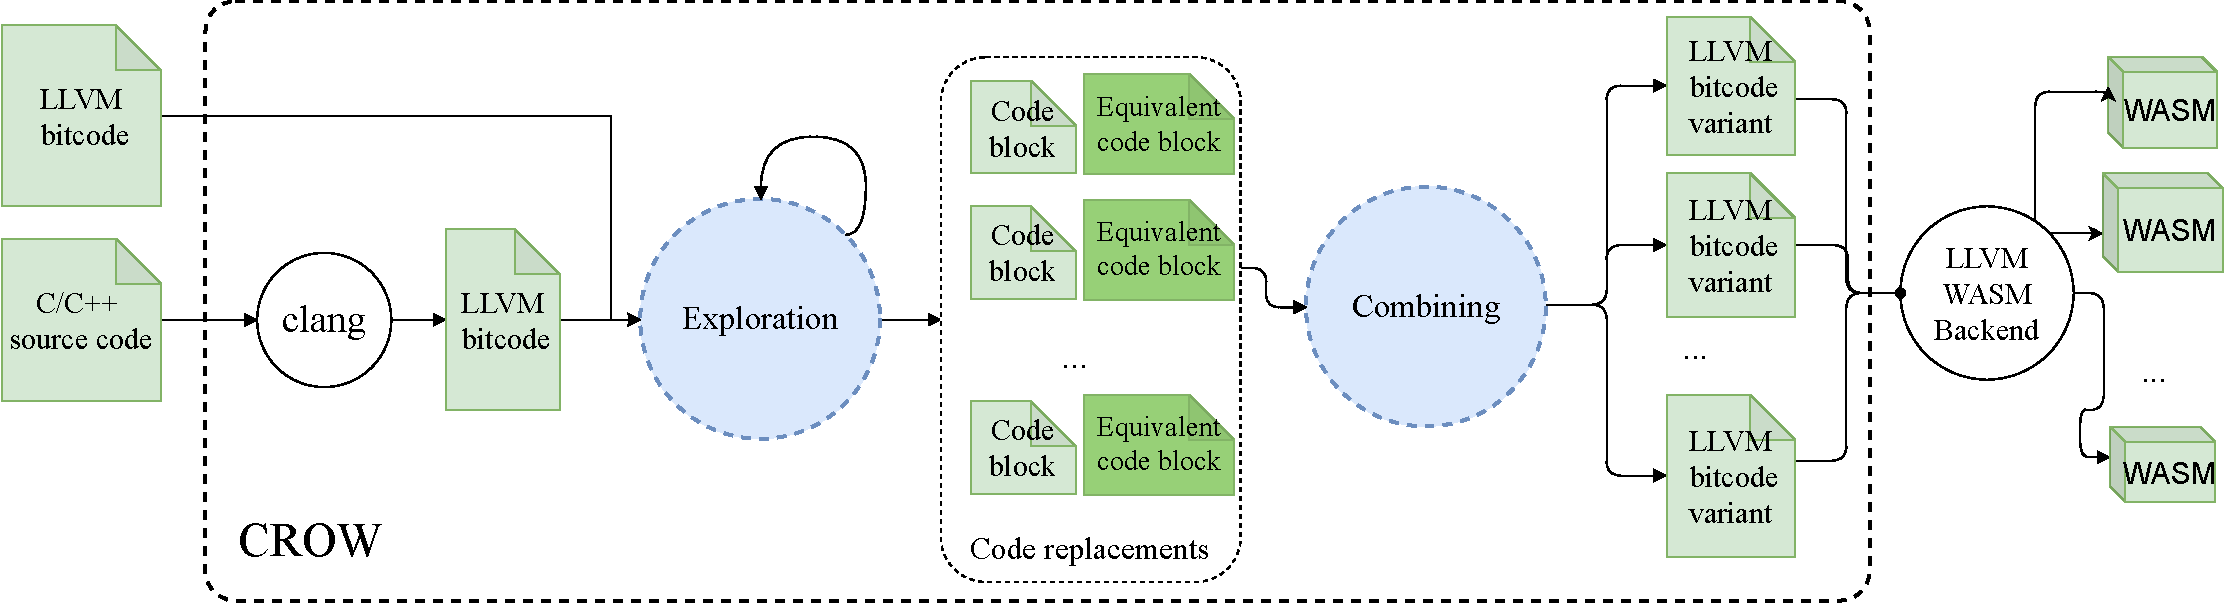
\includegraphics[width=\linewidth]{diagrams/generation/crow.drawio.pdf}
    \caption{CROW workflow to generate program variants. CROW takes C/C++ source codes or LLVM bitcodes to look for code blocks that can be replaced by semantically equivalent code and generates program variants by combining them.}
    \label{diagrams:crow}
\end{figure*}

Figure \ref{diagrams:crow} highlights the main two stages of the CROW's workflow, \textit{exploration} and \textit{combining}. The workflow starts by compiling the input program into the LLVM bitcode using clang from the source code. During the \emph{exploration} stage, CROW takes an LLVM bitcode and, for its code blocks, produces a collection of code replacements that are functionally equivalent to the original program. In the following, we enunciate the definitions we use along with this work for a code block, functional equivalence, and code replacement. 


\begin{definition}{Block (based on Aho \etal \cite{10.5555/6448}):}\label{def:code-block}
    Let $P$ be a program. A block $B$ is a grouping of declarations and statements in $P$ inside a function $F$. 
\end{definition}


\begin{definition}{Functional equivalence modulo program state (based on Le \etal \cite{10.1145/2594291.2594334}):}
    \label{def:functional-equivalence}
    Let $B_1$ and $B_2$ be two code blocks according to \autoref{def:code-block}. We consider the program state before the execution of the block, $S_i$, as the input and the program state after the execution of the block, $S_o$, as the output. $B_1$ and $B_2$ are functionally equivalent if given the same input $S_i$ both codes produce the same output $S_o$.
\end{definition}

\begin{definition}{Code replacement:}
    \label{def:code-replacement}
    Let $P$ be a program and $T$ a pair of code blocks $(B_1, B_2)$. $T$ is a candidate code replacement if $B_1$ and $B_2$ are both functionally equivalent as defined in \autoref{def:functional-equivalence}.
    Applying $T$ to $P$ means replacing $B_1$ by $B_2$. The application of $T$ to $P$ produces a program variant $P'$ which consequently is functionally equivalent to $P$.     
\end{definition}

We implement the \emph{exploration} stage by retargeting a superoptimizer for  LLVM, using its subset of the LLVM intermediate representation. CROW operates at the code block level, taking them from the functions defined inside the input LLVM bitcode module. In addition, the retargeted superoptimizer is in charge of finding the potential places in the original code blocks where a replacement can be applied. Finally, we use the enumerative synthesis strategy of the retargeted superoptimizer to generate code replacements.
The code replacements generated through synthesis are verified, according to \autoref{def:functional-equivalence}, by internally using a theorem prover. 

Moreover, we prevent the superoptimizer from synthesizing instructions that have no correspondence in \wasm for the sake of reducing the searching space for equivalent program variants. Besides, we disable all optimizations in the \wasm LLVM backend that could reverse the superoptimizer transformations, such as constant folding and instructions normalization.

%\todo{We disable cost restrictions and the LLVM backend optimizations...maybe for the assesment RQ ?}

In the \emph{combining} stage, CROW combines the candidate code replacements to generate different LLVM bitcode variants, selecting and merging the code replacements. 
Then for each combination, a variant bitcode is compiled into a \wasm binary if requested. Finally, CROW generates the variants from all possible combinations of code replacements as the power set of all code replacements.  

\end{comment}